\documentclass[margin=2mm]{standalone}
\usepackage{tikz}
\usepackage{amsmath,amssymb,mathtools}
\begin{document}
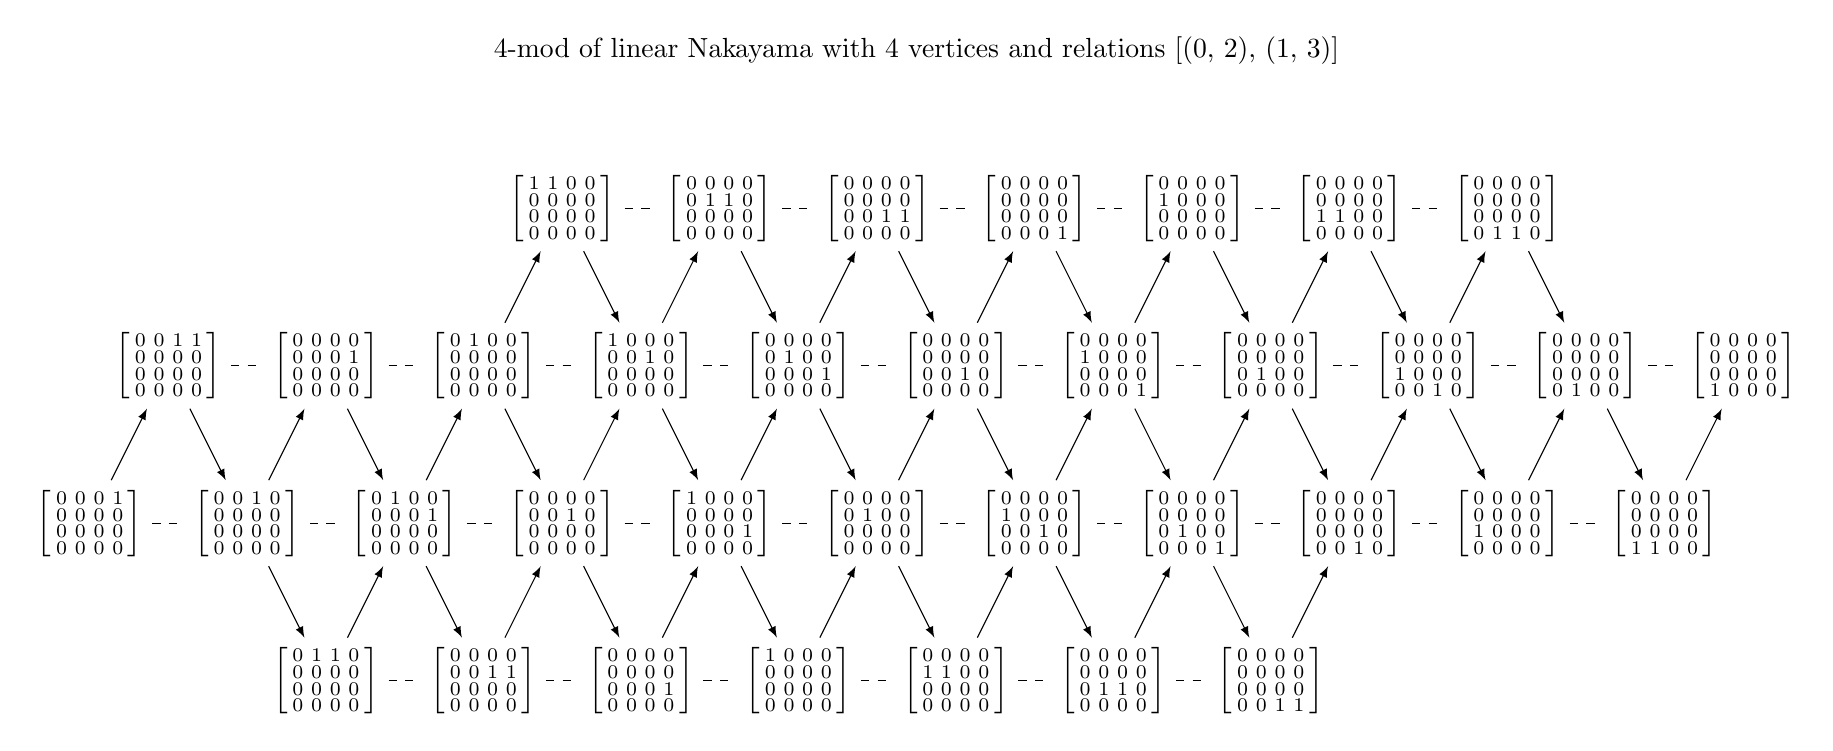
\begin{tikzpicture}[xscale=1,yscale=2]
\node at (10.5,3) [] {$4$-mod of linear Nakayama with 4 vertices and relations [(0, 2), (1, 3)]};
\node (t-0P0) at (6,2) [scale=1] {$\begin{bsmallmatrix}
 1 & 1 & 0 & 0\\
 0 & 0 & 0 & 0\\
 0 & 0 & 0 & 0\\
 0 & 0 & 0 & 0\\
\end{bsmallmatrix}$};
\node (t-1P0) at (8,2) [scale=1] {$\begin{bsmallmatrix}
 0 & 0 & 0 & 0\\
 0 & 1 & 1 & 0\\
 0 & 0 & 0 & 0\\
 0 & 0 & 0 & 0\\
\end{bsmallmatrix}$};
\node (t-2P0) at (10,2) [scale=1] {$\begin{bsmallmatrix}
 0 & 0 & 0 & 0\\
 0 & 0 & 0 & 0\\
 0 & 0 & 1 & 1\\
 0 & 0 & 0 & 0\\
\end{bsmallmatrix}$};
\node (t-3P0) at (12,2) [scale=1] {$\begin{bsmallmatrix}
 0 & 0 & 0 & 0\\
 0 & 0 & 0 & 0\\
 0 & 0 & 0 & 0\\
 0 & 0 & 0 & 1\\
\end{bsmallmatrix}$};
\node (t-4P0) at (14,2) [scale=1] {$\begin{bsmallmatrix}
 0 & 0 & 0 & 0\\
 1 & 0 & 0 & 0\\
 0 & 0 & 0 & 0\\
 0 & 0 & 0 & 0\\
\end{bsmallmatrix}$};
\node (t-5P0) at (16,2) [scale=1] {$\begin{bsmallmatrix}
 0 & 0 & 0 & 0\\
 0 & 0 & 0 & 0\\
 1 & 1 & 0 & 0\\
 0 & 0 & 0 & 0\\
\end{bsmallmatrix}$};
\node (t-6P0) at (18,2) [scale=1] {$\begin{bsmallmatrix}
 0 & 0 & 0 & 0\\
 0 & 0 & 0 & 0\\
 0 & 0 & 0 & 0\\
 0 & 1 & 1 & 0\\
\end{bsmallmatrix}$};
\node (t-0P1) at (3,-1) [scale=1] {$\begin{bsmallmatrix}
 0 & 1 & 1 & 0\\
 0 & 0 & 0 & 0\\
 0 & 0 & 0 & 0\\
 0 & 0 & 0 & 0\\
\end{bsmallmatrix}$};
\node (t-1P1) at (5,-1) [scale=1] {$\begin{bsmallmatrix}
 0 & 0 & 0 & 0\\
 0 & 0 & 1 & 1\\
 0 & 0 & 0 & 0\\
 0 & 0 & 0 & 0\\
\end{bsmallmatrix}$};
\node (t-2P1) at (7,-1) [scale=1] {$\begin{bsmallmatrix}
 0 & 0 & 0 & 0\\
 0 & 0 & 0 & 0\\
 0 & 0 & 0 & 1\\
 0 & 0 & 0 & 0\\
\end{bsmallmatrix}$};
\node (t-3P1) at (9,-1) [scale=1] {$\begin{bsmallmatrix}
 1 & 0 & 0 & 0\\
 0 & 0 & 0 & 0\\
 0 & 0 & 0 & 0\\
 0 & 0 & 0 & 0\\
\end{bsmallmatrix}$};
\node (t-4P1) at (11,-1) [scale=1] {$\begin{bsmallmatrix}
 0 & 0 & 0 & 0\\
 1 & 1 & 0 & 0\\
 0 & 0 & 0 & 0\\
 0 & 0 & 0 & 0\\
\end{bsmallmatrix}$};
\node (t-5P1) at (13,-1) [scale=1] {$\begin{bsmallmatrix}
 0 & 0 & 0 & 0\\
 0 & 0 & 0 & 0\\
 0 & 1 & 1 & 0\\
 0 & 0 & 0 & 0\\
\end{bsmallmatrix}$};
\node (t-6P1) at (15,-1) [scale=1] {$\begin{bsmallmatrix}
 0 & 0 & 0 & 0\\
 0 & 0 & 0 & 0\\
 0 & 0 & 0 & 0\\
 0 & 0 & 1 & 1\\
\end{bsmallmatrix}$};
\node (t-0P2) at (1,1) [scale=1] {$\begin{bsmallmatrix}
 0 & 0 & 1 & 1\\
 0 & 0 & 0 & 0\\
 0 & 0 & 0 & 0\\
 0 & 0 & 0 & 0\\
\end{bsmallmatrix}$};
\node (t-1P2) at (3,1) [scale=1] {$\begin{bsmallmatrix}
 0 & 0 & 0 & 0\\
 0 & 0 & 0 & 1\\
 0 & 0 & 0 & 0\\
 0 & 0 & 0 & 0\\
\end{bsmallmatrix}$};
\node (t-2P2) at (5,1) [scale=1] {$\begin{bsmallmatrix}
 0 & 1 & 0 & 0\\
 0 & 0 & 0 & 0\\
 0 & 0 & 0 & 0\\
 0 & 0 & 0 & 0\\
\end{bsmallmatrix}$};
\node (t-3P2) at (7,1) [scale=1] {$\begin{bsmallmatrix}
 1 & 0 & 0 & 0\\
 0 & 0 & 1 & 0\\
 0 & 0 & 0 & 0\\
 0 & 0 & 0 & 0\\
\end{bsmallmatrix}$};
\node (t-4P2) at (9,1) [scale=1] {$\begin{bsmallmatrix}
 0 & 0 & 0 & 0\\
 0 & 1 & 0 & 0\\
 0 & 0 & 0 & 1\\
 0 & 0 & 0 & 0\\
\end{bsmallmatrix}$};
\node (t-5P2) at (11,1) [scale=1] {$\begin{bsmallmatrix}
 0 & 0 & 0 & 0\\
 0 & 0 & 0 & 0\\
 0 & 0 & 1 & 0\\
 0 & 0 & 0 & 0\\
\end{bsmallmatrix}$};
\node (t-6P2) at (13,1) [scale=1] {$\begin{bsmallmatrix}
 0 & 0 & 0 & 0\\
 1 & 0 & 0 & 0\\
 0 & 0 & 0 & 0\\
 0 & 0 & 0 & 1\\
\end{bsmallmatrix}$};
\node (t-7P2) at (15,1) [scale=1] {$\begin{bsmallmatrix}
 0 & 0 & 0 & 0\\
 0 & 0 & 0 & 0\\
 0 & 1 & 0 & 0\\
 0 & 0 & 0 & 0\\
\end{bsmallmatrix}$};
\node (t-8P2) at (17,1) [scale=1] {$\begin{bsmallmatrix}
 0 & 0 & 0 & 0\\
 0 & 0 & 0 & 0\\
 1 & 0 & 0 & 0\\
 0 & 0 & 1 & 0\\
\end{bsmallmatrix}$};
\node (t-9P2) at (19,1) [scale=1] {$\begin{bsmallmatrix}
 0 & 0 & 0 & 0\\
 0 & 0 & 0 & 0\\
 0 & 0 & 0 & 0\\
 0 & 1 & 0 & 0\\
\end{bsmallmatrix}$};
\node (t-10P2) at (21,1) [scale=1] {$\begin{bsmallmatrix}
 0 & 0 & 0 & 0\\
 0 & 0 & 0 & 0\\
 0 & 0 & 0 & 0\\
 1 & 0 & 0 & 0\\
\end{bsmallmatrix}$};
\node (t-0P3) at (0,0) [scale=1] {$\begin{bsmallmatrix}
 0 & 0 & 0 & 1\\
 0 & 0 & 0 & 0\\
 0 & 0 & 0 & 0\\
 0 & 0 & 0 & 0\\
\end{bsmallmatrix}$};
\node (t-1P3) at (2,0) [scale=1] {$\begin{bsmallmatrix}
 0 & 0 & 1 & 0\\
 0 & 0 & 0 & 0\\
 0 & 0 & 0 & 0\\
 0 & 0 & 0 & 0\\
\end{bsmallmatrix}$};
\node (t-2P3) at (4,0) [scale=1] {$\begin{bsmallmatrix}
 0 & 1 & 0 & 0\\
 0 & 0 & 0 & 1\\
 0 & 0 & 0 & 0\\
 0 & 0 & 0 & 0\\
\end{bsmallmatrix}$};
\node (t-3P3) at (6,0) [scale=1] {$\begin{bsmallmatrix}
 0 & 0 & 0 & 0\\
 0 & 0 & 1 & 0\\
 0 & 0 & 0 & 0\\
 0 & 0 & 0 & 0\\
\end{bsmallmatrix}$};
\node (t-4P3) at (8,0) [scale=1] {$\begin{bsmallmatrix}
 1 & 0 & 0 & 0\\
 0 & 0 & 0 & 0\\
 0 & 0 & 0 & 1\\
 0 & 0 & 0 & 0\\
\end{bsmallmatrix}$};
\node (t-5P3) at (10,0) [scale=1] {$\begin{bsmallmatrix}
 0 & 0 & 0 & 0\\
 0 & 1 & 0 & 0\\
 0 & 0 & 0 & 0\\
 0 & 0 & 0 & 0\\
\end{bsmallmatrix}$};
\node (t-6P3) at (12,0) [scale=1] {$\begin{bsmallmatrix}
 0 & 0 & 0 & 0\\
 1 & 0 & 0 & 0\\
 0 & 0 & 1 & 0\\
 0 & 0 & 0 & 0\\
\end{bsmallmatrix}$};
\node (t-7P3) at (14,0) [scale=1] {$\begin{bsmallmatrix}
 0 & 0 & 0 & 0\\
 0 & 0 & 0 & 0\\
 0 & 1 & 0 & 0\\
 0 & 0 & 0 & 1\\
\end{bsmallmatrix}$};
\node (t-8P3) at (16,0) [scale=1] {$\begin{bsmallmatrix}
 0 & 0 & 0 & 0\\
 0 & 0 & 0 & 0\\
 0 & 0 & 0 & 0\\
 0 & 0 & 1 & 0\\
\end{bsmallmatrix}$};
\node (t-9P3) at (18,0) [scale=1] {$\begin{bsmallmatrix}
 0 & 0 & 0 & 0\\
 0 & 0 & 0 & 0\\
 1 & 0 & 0 & 0\\
 0 & 0 & 0 & 0\\
\end{bsmallmatrix}$};
\node (t-10P3) at (20,0) [scale=1] {$\begin{bsmallmatrix}
 0 & 0 & 0 & 0\\
 0 & 0 & 0 & 0\\
 0 & 0 & 0 & 0\\
 1 & 1 & 0 & 0\\
\end{bsmallmatrix}$};
\draw[-latex] (t-0P0) -- (t-3P2);
\draw[-latex] (t-1P0) -- (t-4P2);
\draw[-latex] (t-2P0) -- (t-5P2);
\draw[-latex] (t-3P0) -- (t-6P2);
\draw[-latex] (t-4P0) -- (t-7P2);
\draw[-latex] (t-5P0) -- (t-8P2);
\draw[-latex] (t-6P0) -- (t-9P2);
\draw[-latex] (t-0P1) -- (t-2P3);
\draw[-latex] (t-1P1) -- (t-3P3);
\draw[-latex] (t-2P1) -- (t-4P3);
\draw[-latex] (t-3P1) -- (t-5P3);
\draw[-latex] (t-4P1) -- (t-6P3);
\draw[-latex] (t-5P1) -- (t-7P3);
\draw[-latex] (t-6P1) -- (t-8P3);
\draw[-latex] (t-0P2) -- (t-1P3);
\draw[-latex] (t-1P2) -- (t-2P3);
\draw[-latex] (t-2P2) -- (t-0P0);
\draw[-latex] (t-2P2) -- (t-3P3);
\draw[-latex] (t-3P2) -- (t-4P3);
\draw[-latex] (t-3P2) -- (t-1P0);
\draw[-latex] (t-4P2) -- (t-5P3);
\draw[-latex] (t-4P2) -- (t-2P0);
\draw[-latex] (t-5P2) -- (t-6P3);
\draw[-latex] (t-5P2) -- (t-3P0);
\draw[-latex] (t-6P2) -- (t-7P3);
\draw[-latex] (t-6P2) -- (t-4P0);
\draw[-latex] (t-7P2) -- (t-8P3);
\draw[-latex] (t-7P2) -- (t-5P0);
\draw[-latex] (t-8P2) -- (t-9P3);
\draw[-latex] (t-8P2) -- (t-6P0);
\draw[-latex] (t-9P2) -- (t-10P3);
\draw[-latex] (t-0P3) -- (t-0P2);
\draw[-latex] (t-1P3) -- (t-0P1);
\draw[-latex] (t-1P3) -- (t-1P2);
\draw[-latex] (t-2P3) -- (t-1P1);
\draw[-latex] (t-2P3) -- (t-2P2);
\draw[-latex] (t-3P3) -- (t-2P1);
\draw[-latex] (t-3P3) -- (t-3P2);
\draw[-latex] (t-4P3) -- (t-3P1);
\draw[-latex] (t-4P3) -- (t-4P2);
\draw[-latex] (t-5P3) -- (t-4P1);
\draw[-latex] (t-5P3) -- (t-5P2);
\draw[-latex] (t-6P3) -- (t-5P1);
\draw[-latex] (t-6P3) -- (t-6P2);
\draw[-latex] (t-7P3) -- (t-6P1);
\draw[-latex] (t-7P3) -- (t-7P2);
\draw[-latex] (t-8P3) -- (t-8P2);
\draw[-latex] (t-9P3) -- (t-9P2);
\draw[-latex] (t-10P3) -- (t-10P2);
\draw[dashed] (t-0P0)--(t-1P0);
\draw[dashed] (t-1P0)--(t-2P0);
\draw[dashed] (t-2P0)--(t-3P0);
\draw[dashed] (t-3P0)--(t-4P0);
\draw[dashed] (t-4P0)--(t-5P0);
\draw[dashed] (t-5P0)--(t-6P0);
\draw[dashed] (t-0P1)--(t-1P1);
\draw[dashed] (t-1P1)--(t-2P1);
\draw[dashed] (t-2P1)--(t-3P1);
\draw[dashed] (t-3P1)--(t-4P1);
\draw[dashed] (t-4P1)--(t-5P1);
\draw[dashed] (t-5P1)--(t-6P1);
\draw[dashed] (t-0P2)--(t-1P2);
\draw[dashed] (t-1P2)--(t-2P2);
\draw[dashed] (t-2P2)--(t-3P2);
\draw[dashed] (t-3P2)--(t-4P2);
\draw[dashed] (t-4P2)--(t-5P2);
\draw[dashed] (t-5P2)--(t-6P2);
\draw[dashed] (t-6P2)--(t-7P2);
\draw[dashed] (t-7P2)--(t-8P2);
\draw[dashed] (t-8P2)--(t-9P2);
\draw[dashed] (t-9P2)--(t-10P2);
\draw[dashed] (t-0P3)--(t-1P3);
\draw[dashed] (t-1P3)--(t-2P3);
\draw[dashed] (t-2P3)--(t-3P3);
\draw[dashed] (t-3P3)--(t-4P3);
\draw[dashed] (t-4P3)--(t-5P3);
\draw[dashed] (t-5P3)--(t-6P3);
\draw[dashed] (t-6P3)--(t-7P3);
\draw[dashed] (t-7P3)--(t-8P3);
\draw[dashed] (t-8P3)--(t-9P3);
\draw[dashed] (t-9P3)--(t-10P3);
\end{tikzpicture}\end{document}